\subsection{Insertion Sort}

Figure \ref{fig:insertion_sort_results} illustrates the time it takes for each language to sort 10'000 positive integers in random order. Note the time differences between Python and the other languages.

\begin{figure}[h]
	\centering
	\mbox{
		\subfigure[Test results from Insertion Sort when run in .NET.]{
			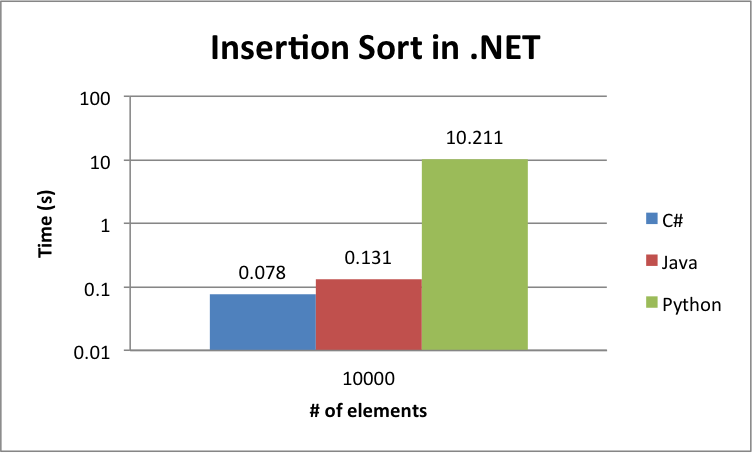
\includegraphics[width=0.48\textwidth]{chapters/media/insertion_sort_all_net.png}
			\label{fig:insertion_sort_all_net}
		}
		\subfigure[Test results from Insertion Sort when run in native environments.]{
			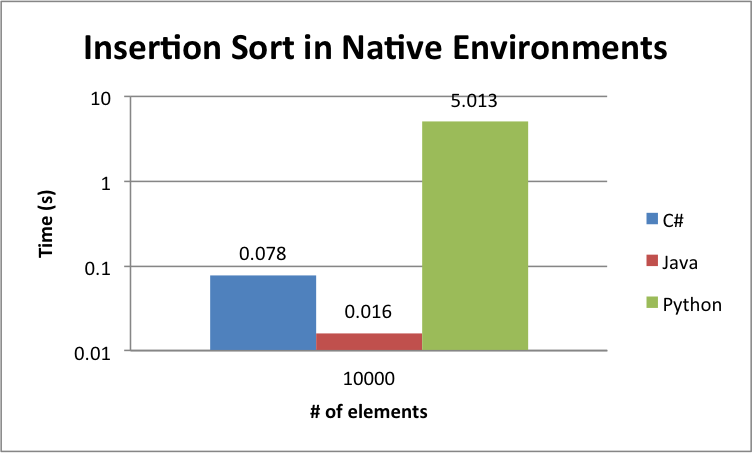
\includegraphics[width=0.48\textwidth]{chapters/media/insertion_sort_all_native.png}
			\label{fig:insertion_sort_all_native}
		}
	}
	\caption{Test results for Insertion Sort in .NET to the left and the native environments to the right.}
	\label{fig:insertion_sort_results}
\end{figure}

Figure \ref{fig:insertion_sort_graphs} illustrates the relation between the number of positive integers in random order (horizontal-axis) and the time (vertical-axis), the graph looks like the expected quadratic curve since the algorithm runs in $O(n^2)$ in its worst case (the perfect curve would require the input to be in reverse order). Note the time difference on the vertical axis when comparing Figure \ref{fig:insertion_sort_csharp_java} and \ref{fig:insertion_sort_python}.

\begin{figure}[h]
	\centering
	\mbox{
		\subfigure[Test results for Insertion Sort in Java and C\#.]{
			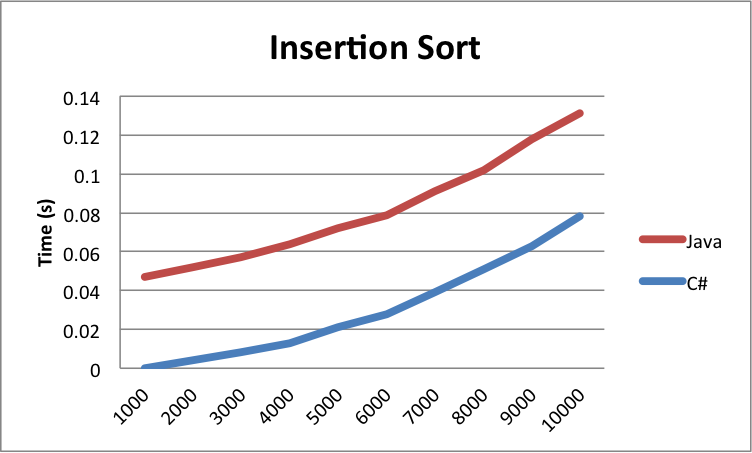
\includegraphics[width=0.48\textwidth]{chapters/media/insertion_sort_csharp_java.png}
			\label{fig:insertion_sort_csharp_java}
		}
		\subfigure[Test results from Insertion Sort in Python.]{
			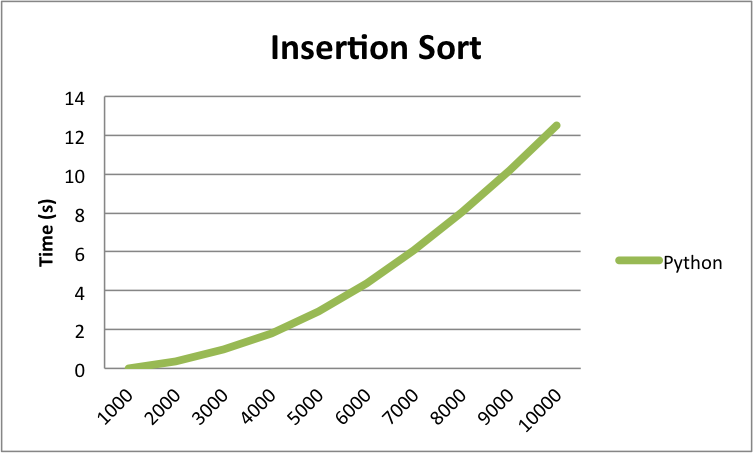
\includegraphics[width=0.48\textwidth]{chapters/media/insertion_sort_python.png}
			\label{fig:insertion_sort_python}
		}
	}
	\caption{Test results for Insertion Sort in C\# and Java to the left and Python to the right.}
	\label{fig:insertion_sort_graphs}
\end{figure} 

\begin{figure}[h]
	\centering
	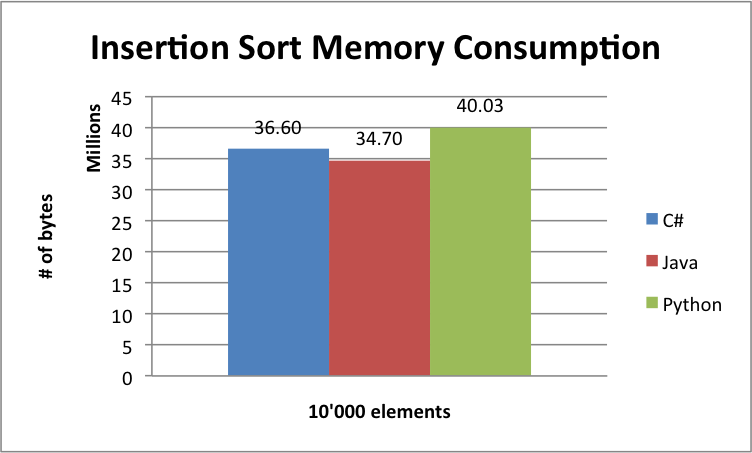
\includegraphics[width=0.6\textwidth]{chapters/media/insertion_sort_memory.png}
	\caption{Comparison of the memory consumption between the three languages run in .NET.}
	\label{fig:insertion_sort_memory}
\end{figure}

The memory consumption was similar for C\# and Java, Python however consumed 30-40\% more (see Figure \ref{fig:insertion_sort_memory}).




















